\documentclass[bigger]{beamer}
\usepackage[spanish, es-tabla]{babel}
\usepackage[utf8]{inputenc}
\usepackage[T1]{fontenc}
\usepackage{xcolor}
\usepackage{amsmath}
\usepackage[absolute,overlay]{textpos}
\usepackage{datetime}
\usepackage[EULERGREEK]{sansmath}
\usepackage{slashbox}
\usepackage{subfig}
\usepackage{tikz}
\usetikzlibrary{shapes, positioning}

\usepackage{graphicx}
\newdate{fecha}{21}{6}{2022}

%%%%%%% Title Page %%%%%%%
\title{Práctica IA de Juegos}
%\subtitle{Subtítulo de la presentación, más largo que el título, pero no mucho}
\date{\displaydate{fecha}}
\author{Sergio Marín Sánchez \\
 José Miguel Sánchez Fernández \\
 Gaspar Muñoz Cava
 }
%\institute{Universidad de Murcia \\ Facultad de Informática}

%Title color
\setbeamercolor*{title}{fg=white}   
%Title size, font family, font weight
\setbeamerfont{title}{size=\LARGE,series=\bfseries,parent=structure,family=\rmfamily} 

%Subtitle color
\setbeamercolor*{subtitle}{fg=white}  
%Subtitle size, font family, font weight
\setbeamerfont{subtitle}{size=\normalsize,series=\bfseries,parent=structure,family=\rmfamily} 

%Caption font
\setbeamerfont{caption name}{family=\rmfamily}
\setbeamercolor{caption name}{fg=black}

%Date color
\setbeamercolor*{date}{fg=white}   

%Author color
\setbeamercolor*{author}{fg=white}  

%Institution color
\setbeamercolor*{institute}{fg=white}  

%Section colors
\setbeamercolor*{section in toc}{fg=white}  
\setbeamercolor*{subsection in toc}{fg=white} 

%Table of contents font size
%\setbeamerfont{section in toc}{size=\scriptsize}

%Table of contents style
\setbeamertemplate{section in toc}[circle]
\setbeamercolor{section number projected}{bg=black}

%%%%%%%%%%%%%%%%%%%%%%%%%%%%

%%%%%%% Global Settings %%%%%%%

%Headers color
\setbeamercolor{frametitle}{fg=white}
%Headers, font family, font weight
\setbeamerfont{frametitle}{size=\Large,series=\bfseries,parent=structure,family=\rmfamily}

%Subheaders color
\setbeamercolor{framesubtitle}{fg=white}
%Subheaders, font family, font weight
\setbeamerfont{framesubtitle}{size=\footnotesize,series=\bfseries,parent=structure,family=\rmfamily}

%Items color
\setbeamercolor{itemize item}{fg=black}

%Background image
\usebackgroundtemplate{
\includegraphics[width=\paperwidth,height=\paperheight]{Fondo3.png}}

%%%%%%%%%%%%%%%%%%%%%%%%%%%%

%%%%%%% Math Settings %%%%%%%

\DeclareMathOperator*{\minimize}{min}
%etc.

%%%%%%%%%%%%%%%%%%%%%%%%%%%%

\begin{document}

%Title Slide
{\usebackgroundtemplate{
\includegraphics[width=\paperwidth]{Fondo1.png}} %Title Background
\begin{frame}
\rmfamily %Title Font
\color{white}\bfseries\maketitle %Title Color & Weight
\end{frame}
}

\newcommand{\RN}[1]{%
  \ensuremath{\textup{\uppercase\expandafter{\romannumeral#1}}}%
}

%Contents Slide
{\usebackgroundtemplate{
\includegraphics[width=\paperwidth]{Fondo2.png}} %Contents Background
\begin{frame}
\frametitle{Índice \RN{1}} %Contents Title
\rmfamily %Contents Font
\color{white}
\tableofcontents[hideallsubsections, sections={1-5}]
\end{frame}
}

%Contents Slide
{\usebackgroundtemplate{
\includegraphics[width=\paperwidth]{Fondo2.png}} %Contents Background
\begin{frame}
\frametitle{Índice \RN{2}} %Contents Title
\rmfamily %Contents Font
\color{white}
\tableofcontents[hideallsubsections, sections={5-}]
\end{frame}
}

\section{Interfaz gráfica}

%Normal Slide (copy, paste and modify this slide for longer presentations)
\begin{frame}[b]
\frametitle{\secname} %Title
\framesubtitle{} %Subtitle
\rmfamily %Font
\color{black} %Color
\begin{figure}
    \centering
    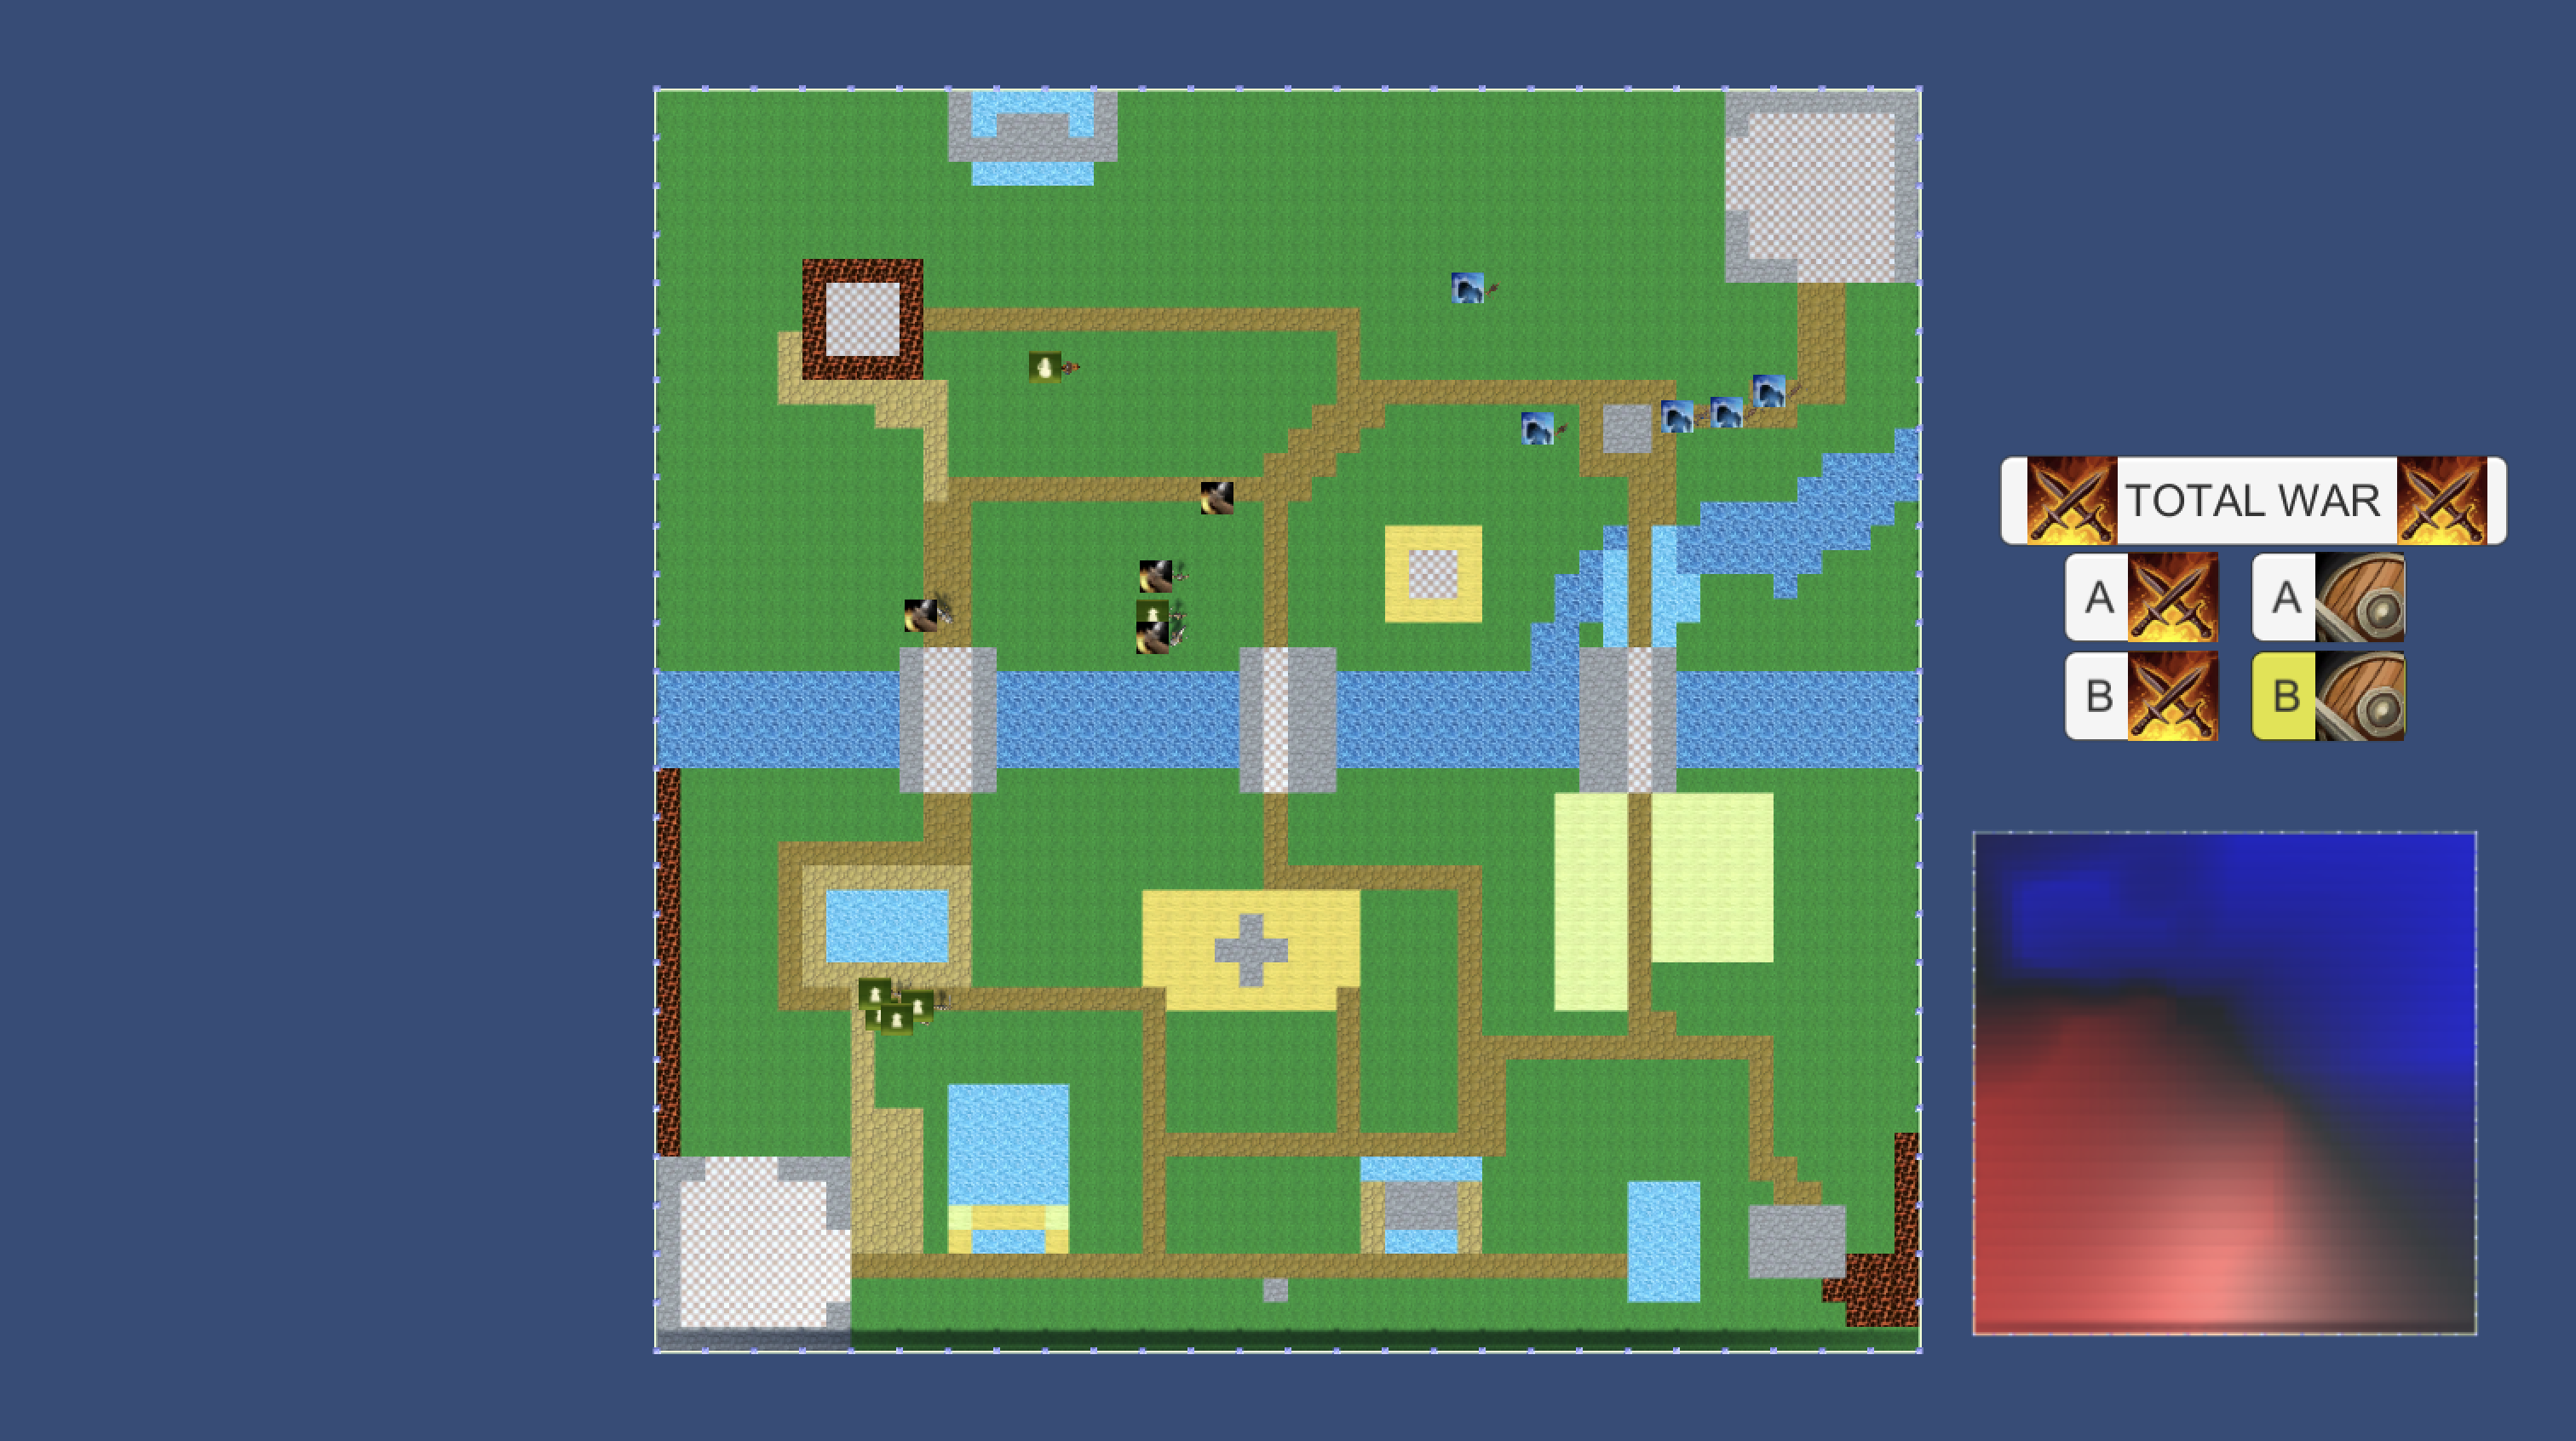
\includegraphics[width=0.9\textwidth]{interfaz.png}
    \caption{Interfaz del juego}
\end{figure}
\end{frame}

\section{Tipos de Unidades}

%Normal Slide (copy, paste and modify this slide for longer presentations)
\begin{frame}[b]
\frametitle{\secname} %Title
\framesubtitle{} %Subtitle
\rmfamily %Font
\color{black} %Color
\begin{table}
    \centering
    \resizebox{0.7\textwidth}{!}{
    \begin{tabular}{|c|c|c|c|c|c|}
        \cline{2-5}        
        \multicolumn{1}{c|}{} & 
\includegraphics{../doc/imagesTable/infanteria} & 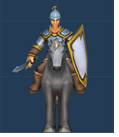
\includegraphics{../doc/imagesTable/caballo} & 
\includegraphics{../doc/imagesTable/lancero} & 
\includegraphics{../doc/imagesTable/arquero} & \multicolumn{1}{|c}{} \\
        \hline
        
\includegraphics{../doc/imagesTable/claroPiedra} 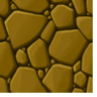
\includegraphics{../doc/imagesTable/piedra} 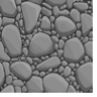
\includegraphics{../doc/imagesTable/grisPiedra} & \backslashbox{1.5}{75} & \backslashbox{1.5}{75} & \backslashbox{1.5}{90} & \backslashbox{1.5}{90} & \backslashbox{Coste}{Factor (\%)} \\
        \hline
        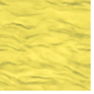
\includegraphics{../doc/imagesTable/arena} 
\includegraphics{../doc/imagesTable/claroArena} & \backslashbox{10}{25} & \backslashbox{10}{25} & \backslashbox{3}{60} & \backslashbox{3}{60} & \backslashbox{Coste}{Factor (\%)} \\
        \hline
        
\includegraphics{../doc/imagesTable/agua} 
\includegraphics{../doc/imagesTable/claroAgua} & \backslashbox{$\infty$}{0} & \backslashbox{$\infty$}{0} & \backslashbox{$\infty$}{0} & \backslashbox{$\infty$}{0} & \backslashbox{Coste}{Factor (\%)} \\
        \hline
        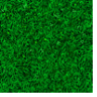
\includegraphics{../doc/imagesTable/hierba} & \backslashbox{5}{50} & \backslashbox{1}{100} & \backslashbox{5}{45} & \backslashbox{1}{100} & \backslashbox{Coste}{Factor (\%)} \\
        \hline
        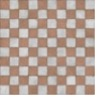
\includegraphics[scale=0.33]{../doc/imagesTable/suelo} & \backslashbox{1}{100} & \backslashbox{5}{50} & \backslashbox{1}{100} & \backslashbox{1}{100} & \backslashbox{Coste}{Factor (\%)} \\
        \hline
        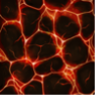
\includegraphics{../doc/imagesTable/lava} & \backslashbox{15}{5} & \backslashbox{15}{5} & \backslashbox{15}{10} & \backslashbox{15}{2} & \backslashbox{Coste}{Factor (\%)} \\
        \hline
    \end{tabular}
    }
    \caption{Tabla de coste de influencias y factores de velocidad}
\end{table}
\end{frame}

\section{Comportamiento estratégico}

%Normal Slide (copy, paste and modify this slide for longer presentations)
\begin{frame}
\frametitle{\secname} %Title
\framesubtitle{} %Subtitle
\rmfamily %Font
\color{black} %Color
\begin{figure}[b]
    \centering
    \newcommand{\behaviourmodes}{../IA_Juegos/Assets/Textures/UI}
\begin{tikzpicture}
    \sffamily\sansmath
    \node[draw, rounded corners, minimum width = 5cm, minimum height = 1cm, fill = white] (0) {TOTAL WAR};
    \node (1) [right = -1.3cm of 0] {
\includegraphics[scale=0.11]{\behaviourmodes/AttackMode}};
    \node (2) [left = -1.3cm of 0] {
\includegraphics[scale=0.11]{\behaviourmodes/AttackMode}};
    
    \node[draw, align = left, rounded corners, minimum width = 1.5cm, minimum height = 1cm, fill = white] (3) at (-1.1, -1.1) {\phantom{l}A\phantom{llllllllllll}};
    \node (4) [right = -1.3cm of 3] {
\includegraphics[scale=0.11]{\behaviourmodes/AttackMode}};
    
    \node[draw, align = left, rounded corners, minimum width = 1.5cm, minimum height = 1cm, fill = white] (5) at (1.1, -1.1) {\phantom{l}A\phantom{llllllllllll}};
    \node (6) [right = -1.3cm of 5] {
\includegraphics[scale=0.11]{\behaviourmodes/DefenseMode}};
    
    \node[draw, align = left, rounded corners, minimum width = 1.5cm, minimum height = 1cm, fill = white] (7) at (-1.1, -2.2) {\phantom{l}B\phantom{llllllllllll}};
    \node (8) [right = -1.3cm of 7] {
\includegraphics[scale=0.11]{\behaviourmodes/AttackMode}};
    
    \node[draw, align = left, rounded corners, minimum width = 1.5cm, minimum height = 1cm, fill = white] (9) at (1.1, -2.2) {\phantom{l}B\phantom{llllllllllll}};
    \node (10) [right = -1.3cm of 9] {
\includegraphics[scale=0.11]{\behaviourmodes/DefenseMode}};
\end{tikzpicture}
    \caption{Botones de cambio de modo}
\end{figure}
\end{frame}

\section{Modo Debug}

%Normal Slide (copy, paste and modify this slide for longer presentations)
\begin{frame}[b]
\frametitle{\secname} %Title
\framesubtitle{} %Subtitle
\rmfamily %Font
\color{black} %Color
\begin{figure}[b!]
    \centering
    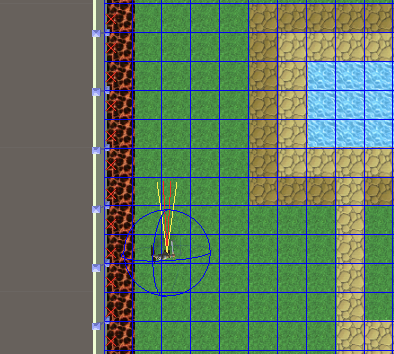
\includegraphics[width=0.6\textwidth]{debug.png}
    \caption{Variables del personaje}
\end{figure}
\end{frame}

\section{Comportamiento táctico}

\subsection{Unidad de infantería}

%Normal Slide (copy, paste and modify this slide for longer presentations)
\begin{frame}
\frametitle{\secname} %Title
\framesubtitle{\subsecname} %Subtitle
\rmfamily %Font
\color{black} %Color
\begin{figure}[b]
    \centering
    \resizebox{0.7\textwidth}{!}{
        \begin{tikzpicture}
            \node (0) {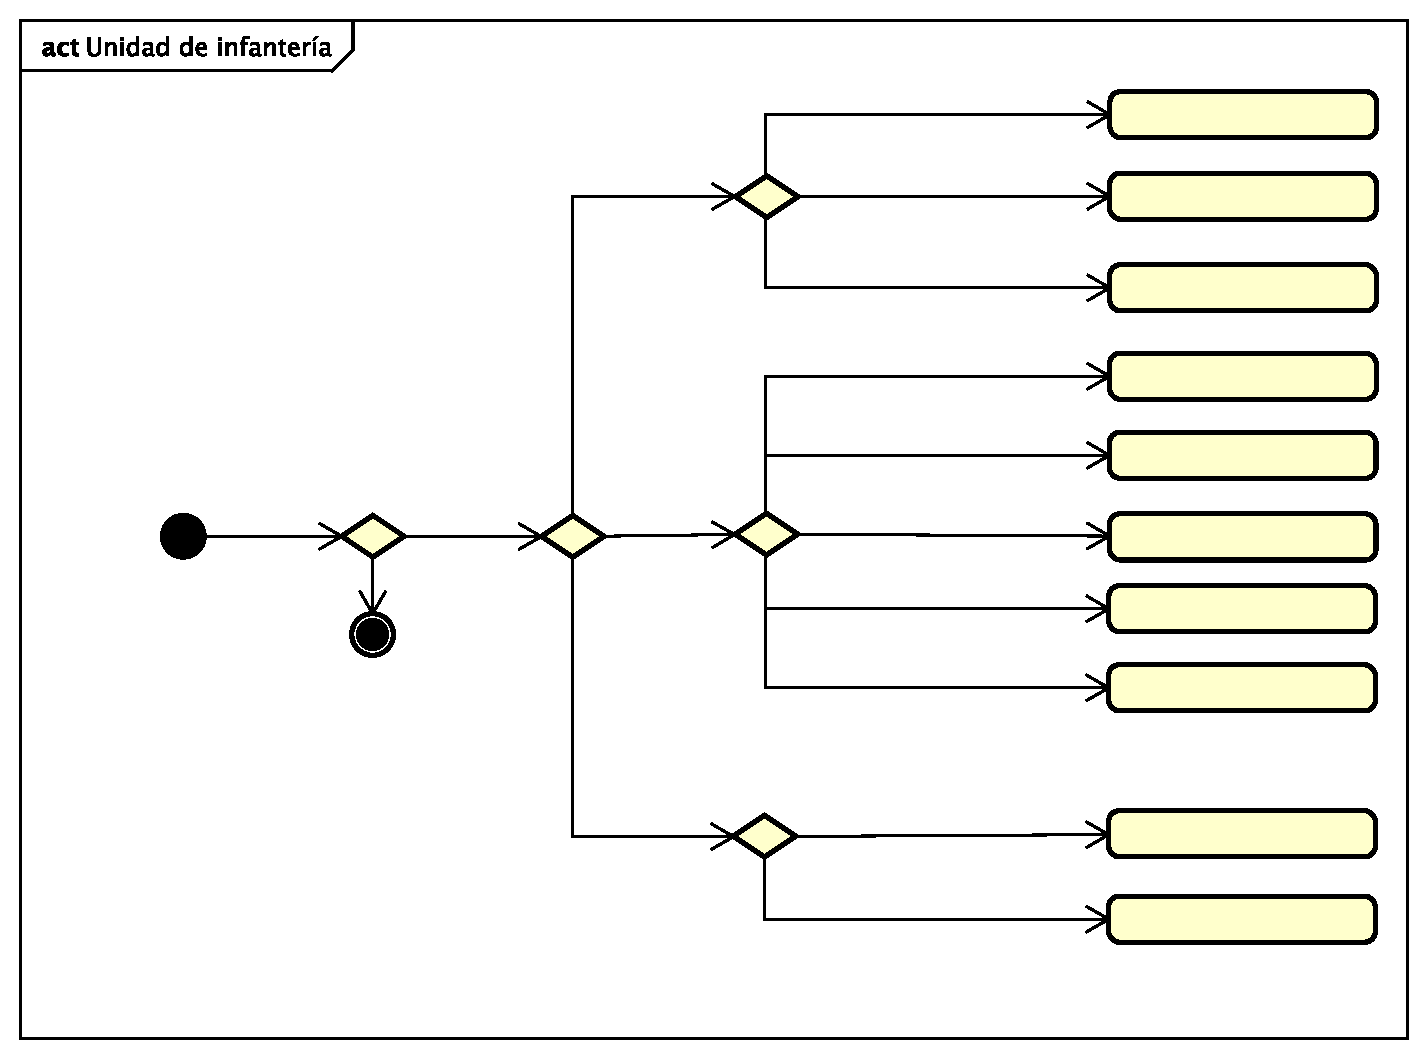
\includegraphics{../doc/behaviourTrees/pdfs/arbolInfanteria}};
            \node (1) at (-6.3,-0.75) {No};
            \node (2) at (-4.9,0.2) {Sí};
            \node (3) at (-6.5,0.3) {¿Vivo?};
            \node (4) at (-3.3,0.4) {¿Estado?};
            \node (5) at (-1.3,6) {Guerra Total};
            \node (6) at (-1.3,0.2) {Ataque};
            \node (7) at (-1.3,-4.9) {Defensa};
            
            \node (8) at (3,6) {¿Enemigo cerca?};
            \node (9) at (3,7.3) {¿En base enemiga?};
            \node (10) at (9,5.6) {Atacar enemigo};
            \node (11) at (9,7) {Capturar base enemiga};
            \node (12) at (9,4.1) {Ir a la base enemiga};
            
            \node (13) at (3,1.6) {¿Enemigo cerca?};
            \node (14) at (3,2.9) {¿En base enemiga?};
            \node[text width = 4.35cm] (14) at (3.75,0.2) {¿En el punto de curación y  no todos puntos de vida?};
            \node (16) at (3.4,-1.1) {¿Pocos puntos de vida?};
            \node (17) at (9,1.25) {Atacar enemigo};
            \node (18) at (9,2.6) {Capturar base enemiga};
            \node (19) at (9,-2.7) {Ir a la base enemiga};
            \node (20) at (9,-0.1) {Curarse};
            \node (21) at (9,-1.35) {Ir al punto de curación};
            
            \node (22) at (3,-4.9) {¿Enemigo cerca?};
            \node (23) at (9,-5.15) {Atacar enemigo};
            \node (24) at (9,-6.6) {Defender};
        \end{tikzpicture}
    }
    \caption{Árbol de comportamiento de infantería pesada}
    \label{fig:infantery}
\end{figure}

\end{frame}

\subsection{Unidad lancero}

%Normal Slide (copy, paste and modify this slide for longer presentations)
\begin{frame}
\frametitle{\secname} %Title
\framesubtitle{\subsecname} %Subtitle
\rmfamily %Font
\color{black} %Color
\begin{figure}[b]
    \centering
    \resizebox{0.7\textwidth}{!}{
        \begin{tikzpicture}
            \node (0) {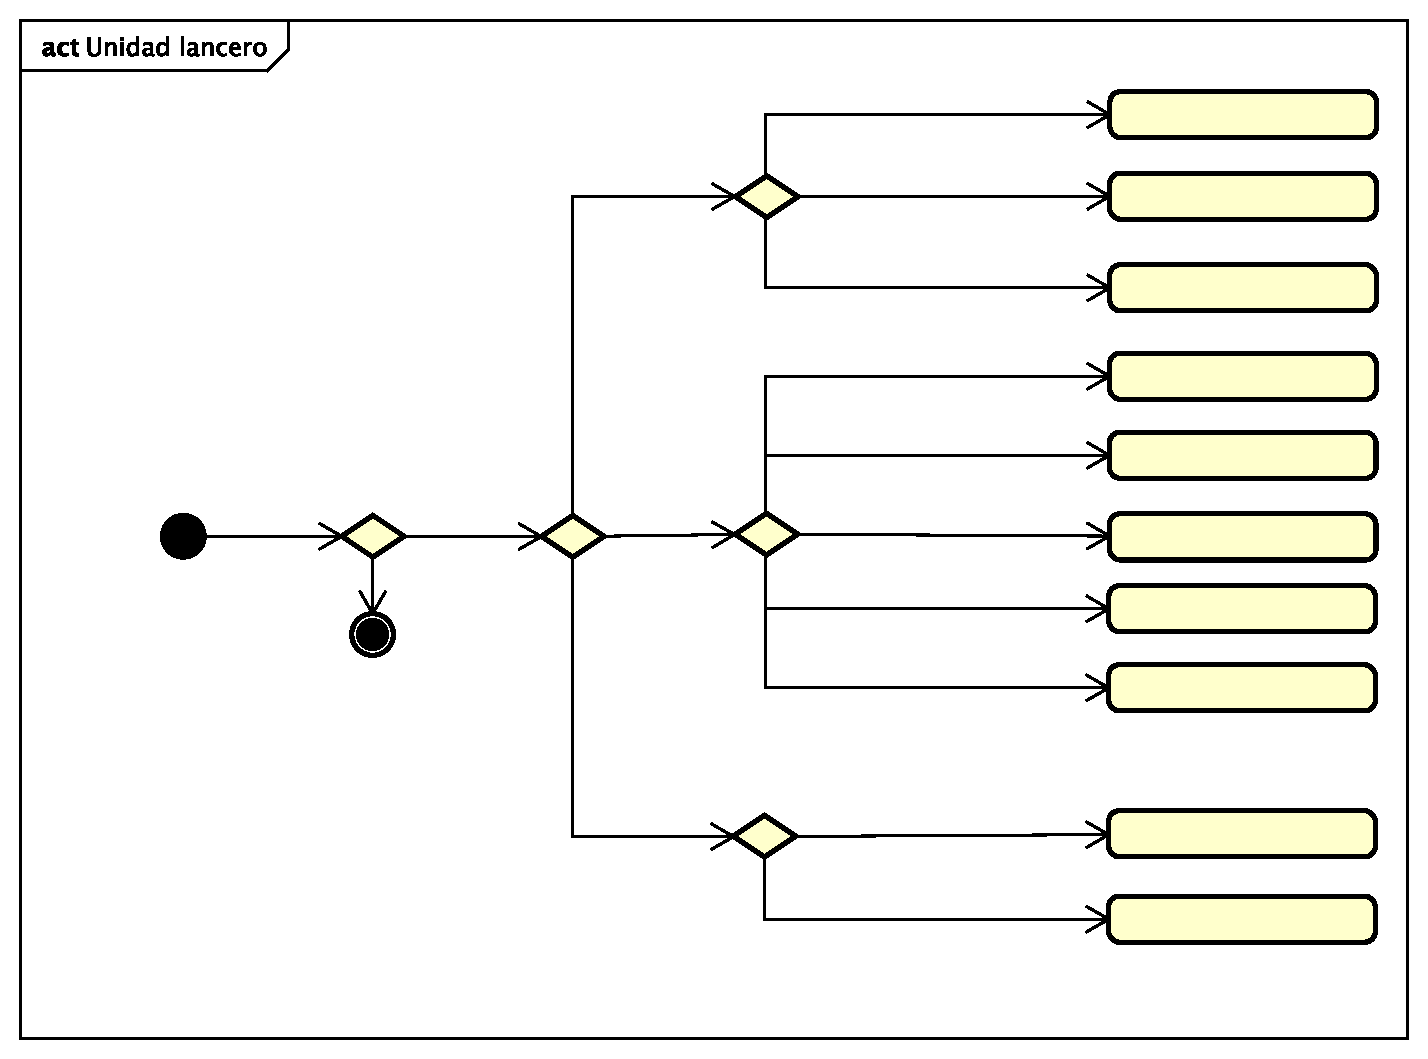
\includegraphics{../doc/behaviourTrees/pdfs/arbolLancero}};
            \node (1) at (-6.3,-0.75) {No};
            \node (2) at (-4.9,0.2) {Sí};
            \node (3) at (-6.5,0.3) {¿Vivo?};
            \node (4) at (-3.3,0.4) {¿Estado?};
            \node (5) at (-1.3,6) {Guerra Total};
            \node (6) at (-1.3,0.2) {Ataque};
            \node (7) at (-1.3,-4.9) {Defensa};
            
            \node (8) at (3,6) {¿En base enemiga?};
            \node (9) at (3,7.3) {¿Enemigo cerca?};
            \node (10) at (9,5.6) {Capturar base enemiga};
            \node (11) at (9,7) {Atacar enemigo};
            \node (12) at (9,4.1) {Ir a la base enemiga};
            
            \node (13) at (3,2.9) {¿Enemigo cerca?};
            \node (14) at (3.2,0.2) {¿En base enemiga?}; 
            \node[text width = 4.35cm] (14) at (3.75,1.6) {¿En el punto de curación y  no todos puntos de vida?}; 
            \node (16) at (3,-1.1) {¿Pocos puntos de vida?};
            \node (17) at (9,1.25) {Curarse};
            \node (18) at (9,2.6) {Atacar enemigo};
            \node (19) at (9,-2.7) {Ir a la base enemiga};
            \node (20) at (9,-0.1) {Capturar base enemiga};
            \node (21) at (9,-1.35) {Ir al punto de curación};
            
            \node (22) at (3,-4.9) {¿Enemigo cerca?};
            \node (23) at (9,-5.15) {Atacar enemigo};
            \node (24) at (9,-6.6) {Defender};
        \end{tikzpicture}
    }
    \caption{Árbol de comportamiento de lancero}
    \label{fig:lancer}
\end{figure}
\end{frame}

\subsection{Unidad arquero}

%Normal Slide (copy, paste and modify this slide for longer presentations)
\begin{frame}
\frametitle{\secname} %Title
\framesubtitle{\subsecname} %Subtitle
\rmfamily %Font
\color{black} %Color
\begin{figure}[b]
    \centering
    \resizebox{0.7\textwidth}{!}{
        \begin{tikzpicture}
            \node (0) {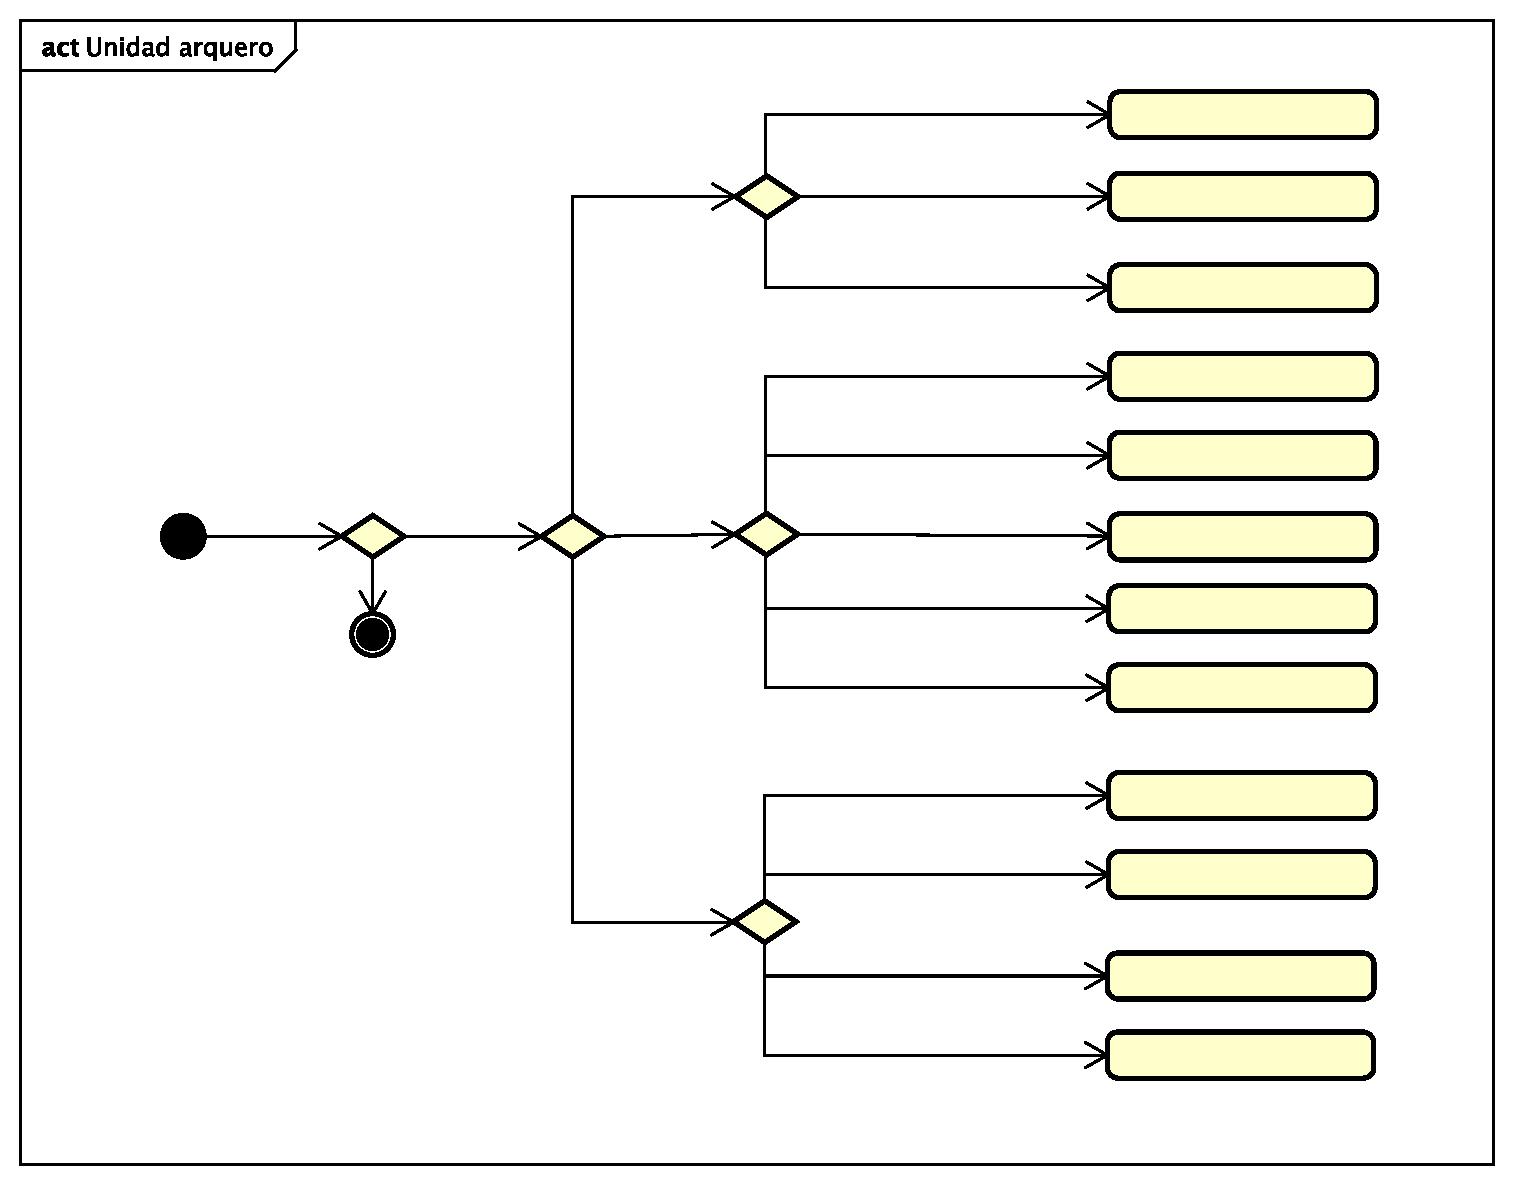
\includegraphics{../doc/behaviourTrees/pdfs/arbolArquero}};
            \node (1) at (-6.9,0.35) {No};
            \node (2) at (-5.5,1.2) {Sí};
            \node (3) at (-7.3,1.3) {¿Vivo?};
            \node (4) at (-4,1.4) {¿Estado?};
            \node (5) at (-2,7) {Guerra Total};
            \node (6) at (-2,1.2) {Ataque};
            \node (7) at (-2,-5.3) {Defensa};
            
            \node (8) at (3,7) {¿En base enemiga?};
            \node (9) at (3,8.3) {¿Enemigo cerca?};
            \node (10) at (8.2,6.6) {Capturar base enemiga};
            \node (11) at (8.2,8) {Atacar enemigo};
            \node (12) at (8.2,5.1) {Ir a la base enemiga};
            
            \node (13) at (3,1.2) {¿Enemigo cerca?};
            \node (14) at (3.2,0) {¿En base enemiga?}; 
            \node[text width = 4.35cm] (14) at (3,4) {¿En el punto de curación y  no todos puntos de vida?}; 
            \node (16) at (3,2.6) {¿Pocos puntos de vida?};
            \node (17) at (8.2,3.7) {Curarse};
            \node (18) at (8.2 ,0.9) {Atacar enemigo};
            \node (19) at (8.2 ,-1.6) {Ir a la base enemiga};
            \node (20) at (8.2, -0.3) {Capturar base enemiga};
            \node (21) at (8.2, 2.3) {Ir al punto de curación};
            
            \node (22) at (3, -4.5) {¿Pocos puntos de vida?};
            \node[text width = 4.35cm] (23) at (3,-3.2) {¿En el punto de curación y  no todos puntos de vida?}; 
            \node (24) at (3, -6.2) {¿Enemigo cerca?};
            \node (25) at (8.2, -6.5) {Atacar enemigo};
            \node (26) at (8.2, -7.8) {Defender};
            \node (25) at (8.2, -3.4) {Curarse};
            \node (26) at (8.2, -4.8) {Ir al punto de curación};
        \end{tikzpicture}
    }
    \caption{Árbol de comportamiento de arquero}
    \label{fig:archer}
\end{figure}
\end{frame}

\subsection{Unidad de caballería}

%Normal Slide (copy, paste and modify this slide for longer presentations)
\begin{frame}
\frametitle{\secname} %Title
\framesubtitle{\subsecname} %Subtitle
\rmfamily %Font
\color{black} %Color
\begin{figure}[b]
    \centering
    \resizebox{0.7\textwidth}{!}{
        \begin{tikzpicture}
            \node (0) {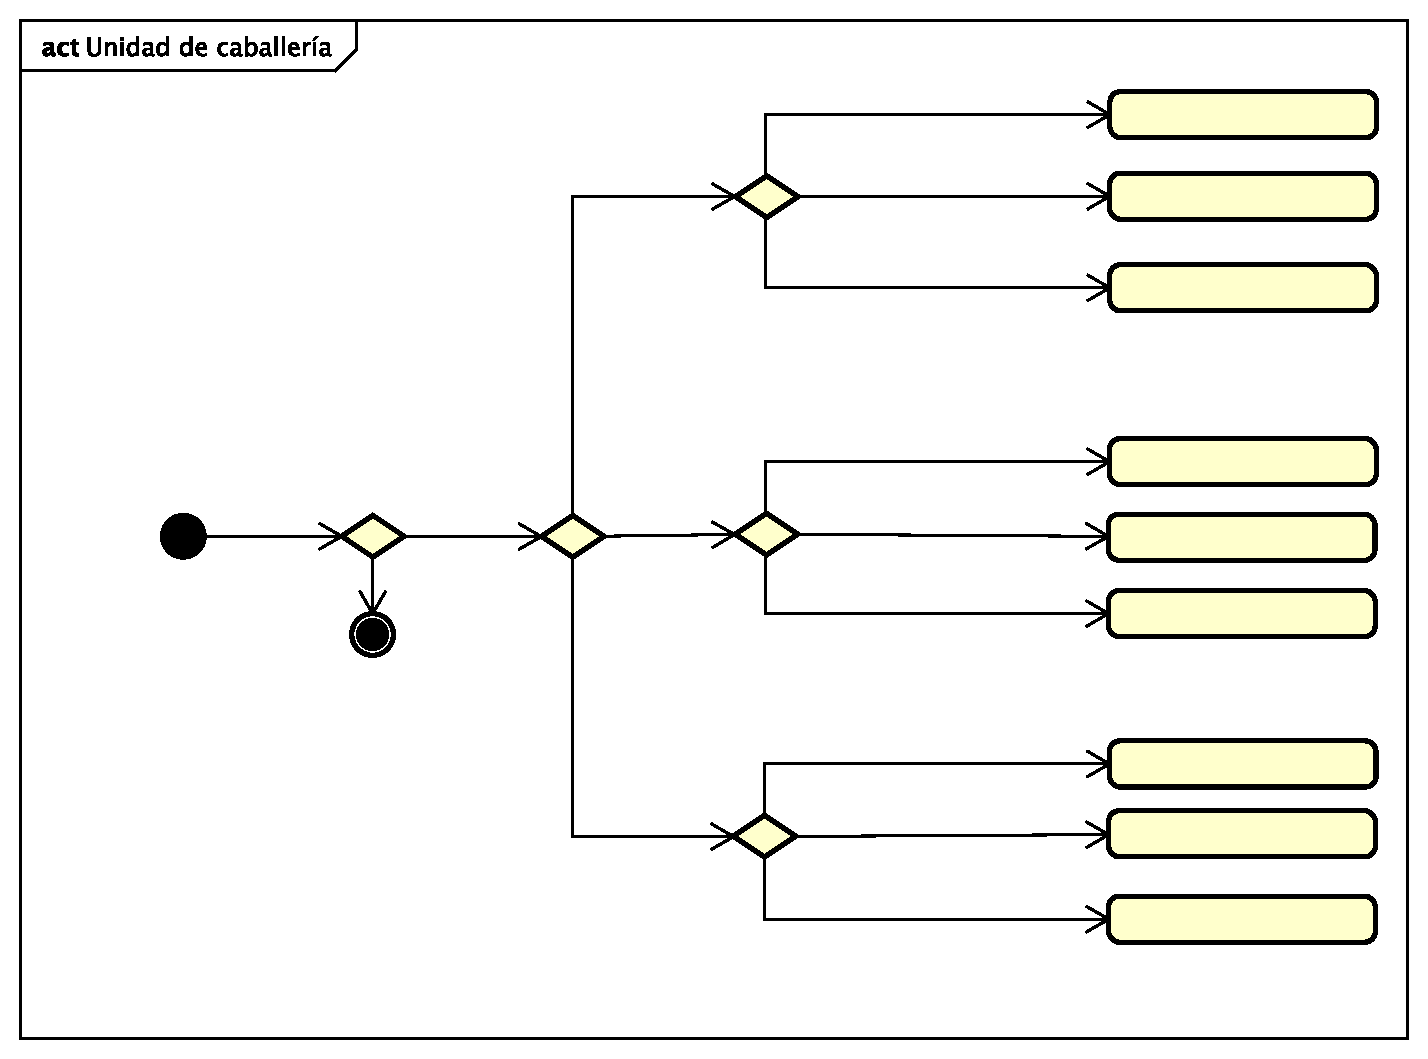
\includegraphics{../doc/behaviourTrees/pdfs/arbolCaballo}};
            \node (1) at (-6.3,-0.75) {No};
            \node (2) at (-4.9,0.2) {Sí};
            \node (3) at (-6.5,0.3) {¿Vivo?};
            \node (4) at (-3.3,0.4) {¿Estado?};
            \node (5) at (-1.3,6) {Guerra Total};
            \node (6) at (-1.3,0.2) {Ataque};
            \node (7) at (-1.3,-4.9) {Defensa};
            
            \node (8) at (3,6) {¿En base enemiga?};
            \node (9) at (3,7.3) {¿Enemigo cerca?};
            \node (10) at (9,5.6) {Capturar base enemiga};
            \node (11) at (9,7) {Atacar enemigo};
            \node (12) at (9,4.1) {Ir a la base enemiga};
            
            \node (14) at (3.75,1.5) {¿Enemigo Cerca?}; 
            \node (17) at (9,1.25) {Atacar enemigo};
            \node (27) at (3.75,0.2) {¿Lejos de la base?}; 
            \node (28) at (9,0) {Defender};
            \node (29) at (3.75,-1.1) {¿Cerca de la base?}; 
            \node (21) at (9,-1.4) {Ir a la base enemiga};
            
            \node (22) at (3,-3.7) {¿Enemigo cerca?};
            \node (23) at (9,-3.9) {Atacar enemigo};
            \node (25) at (3,-4.9) {¿Lejos de la base?};
            \node (26) at (9,-5.15) {Defender};
            \node (24) at (9,-6.6) {Ir al punto de curación};
        \end{tikzpicture}
    }
    \caption{Árbol de comportamiento de caballería}
    \label{fig:horse}
\end{figure}
\end{frame}

\section{Sistema de combate}

%Normal Slide (copy, paste and modify this slide for longer presentations)
\begin{frame}
\frametitle{\secname} %Title
\framesubtitle{} %Subtitle
\rmfamily %Font
\color{black} %Color
\begin{table}[b]
    \centering
    \resizebox{\textwidth}{!}{
    \begin{tabular}{|c|c|c|c|c|}
       \hline        
       \textbf{Unidad} & Daño base & Rango de ataque & Velocidad de ataque & Vida máxima \\
        \hline
        Lancero & 40 & 6 & 4 & 250 \\
        \hline
        Infantería & 10 & 6 & 4 & 200 \\
        \hline
        Caballería & 30 & 6 & 4 & 130 \\
        \hline
        Arquero & 20 & 14 & 4 & 100 \\
        \hline
    \end{tabular}
    }
    \caption{Tabla de Influencias}
\end{table}
\end{frame}

\section{Mapa Táctico}

\subsection{Mapa de influencia}

%Normal Slide (copy, paste and modify this slide for longer presentations)
\begin{frame}
\frametitle{\secname} %Title
\framesubtitle{\subsecname} %Subtitle
\rmfamily %Font
\color{black} %Color
\begin{columns}
\column{0.45\textwidth}
\begin{figure}
    \centering
    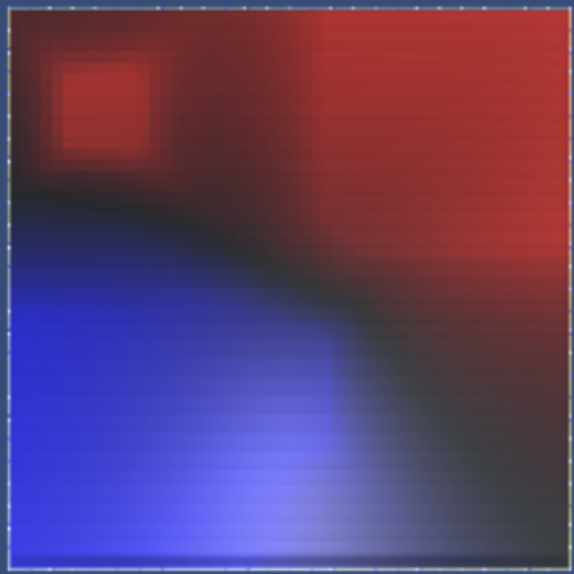
\includegraphics[width=0.6\textwidth]{../doc/images/InfluenciaMap.png}
    \caption{Mapa de Influencia}
\end{figure}
\column{0.7\textwidth}
\begin{gather*}
    Influencia_{i,j} = \frac{Influencia_{base}}{\left(1 + d\left((i,j), (x,y)\right)\right)^{1.25}}
\end{gather*}
\begin{gather*}
    d\left((i,j), (x,y)\right) = \max \left( \lvert x - i \rvert, \lvert y - j \rvert \right)
\end{gather*}
\end{columns}
\end{frame}

\subsection{Mapas de Tensión y Vulnerabilidad}

%Normal Slide (copy, paste and modify this slide for longer presentations)
\begin{frame}
\frametitle{\secname} %Title
\framesubtitle{\subsecname} %Subtitle
\rmfamily %Font
\color{black} %Color
\begin{columns}
\column{0.45\textwidth}
\begin{figure}
    \centering
    \subfloat{
\includegraphics[width=0.6\textwidth]{../doc/images/TensionMap.png}} \\
    \subfloat{\includegraphics[width=0.6\textwidth]{../doc/images/vulnerabilidadMap.png}}
    \caption{Mapas de tensión y vulnerabilidad}
\end{figure}
\column{0.7\textwidth}
\begin{gather*}
    Tension = \frac{Influencia_A + Influencia_B}{2}
\end{gather*}
\vspace{1.5cm}
\begin{gather*}
    Vulnerabilidad = Tension - \lvert Influencia \rvert
\end{gather*}
\vspace{0.6cm}
\end{columns}
\end{frame}

\section{Pathfinding táctico individual}

%Normal Slide (copy, paste and modify this slide for longer presentations)
\begin{frame}[b]
\frametitle{\secname} %Title
\framesubtitle{} %Subtitle
\rmfamily %Font
\color{black} %Color
\begin{figure}
    \centering
    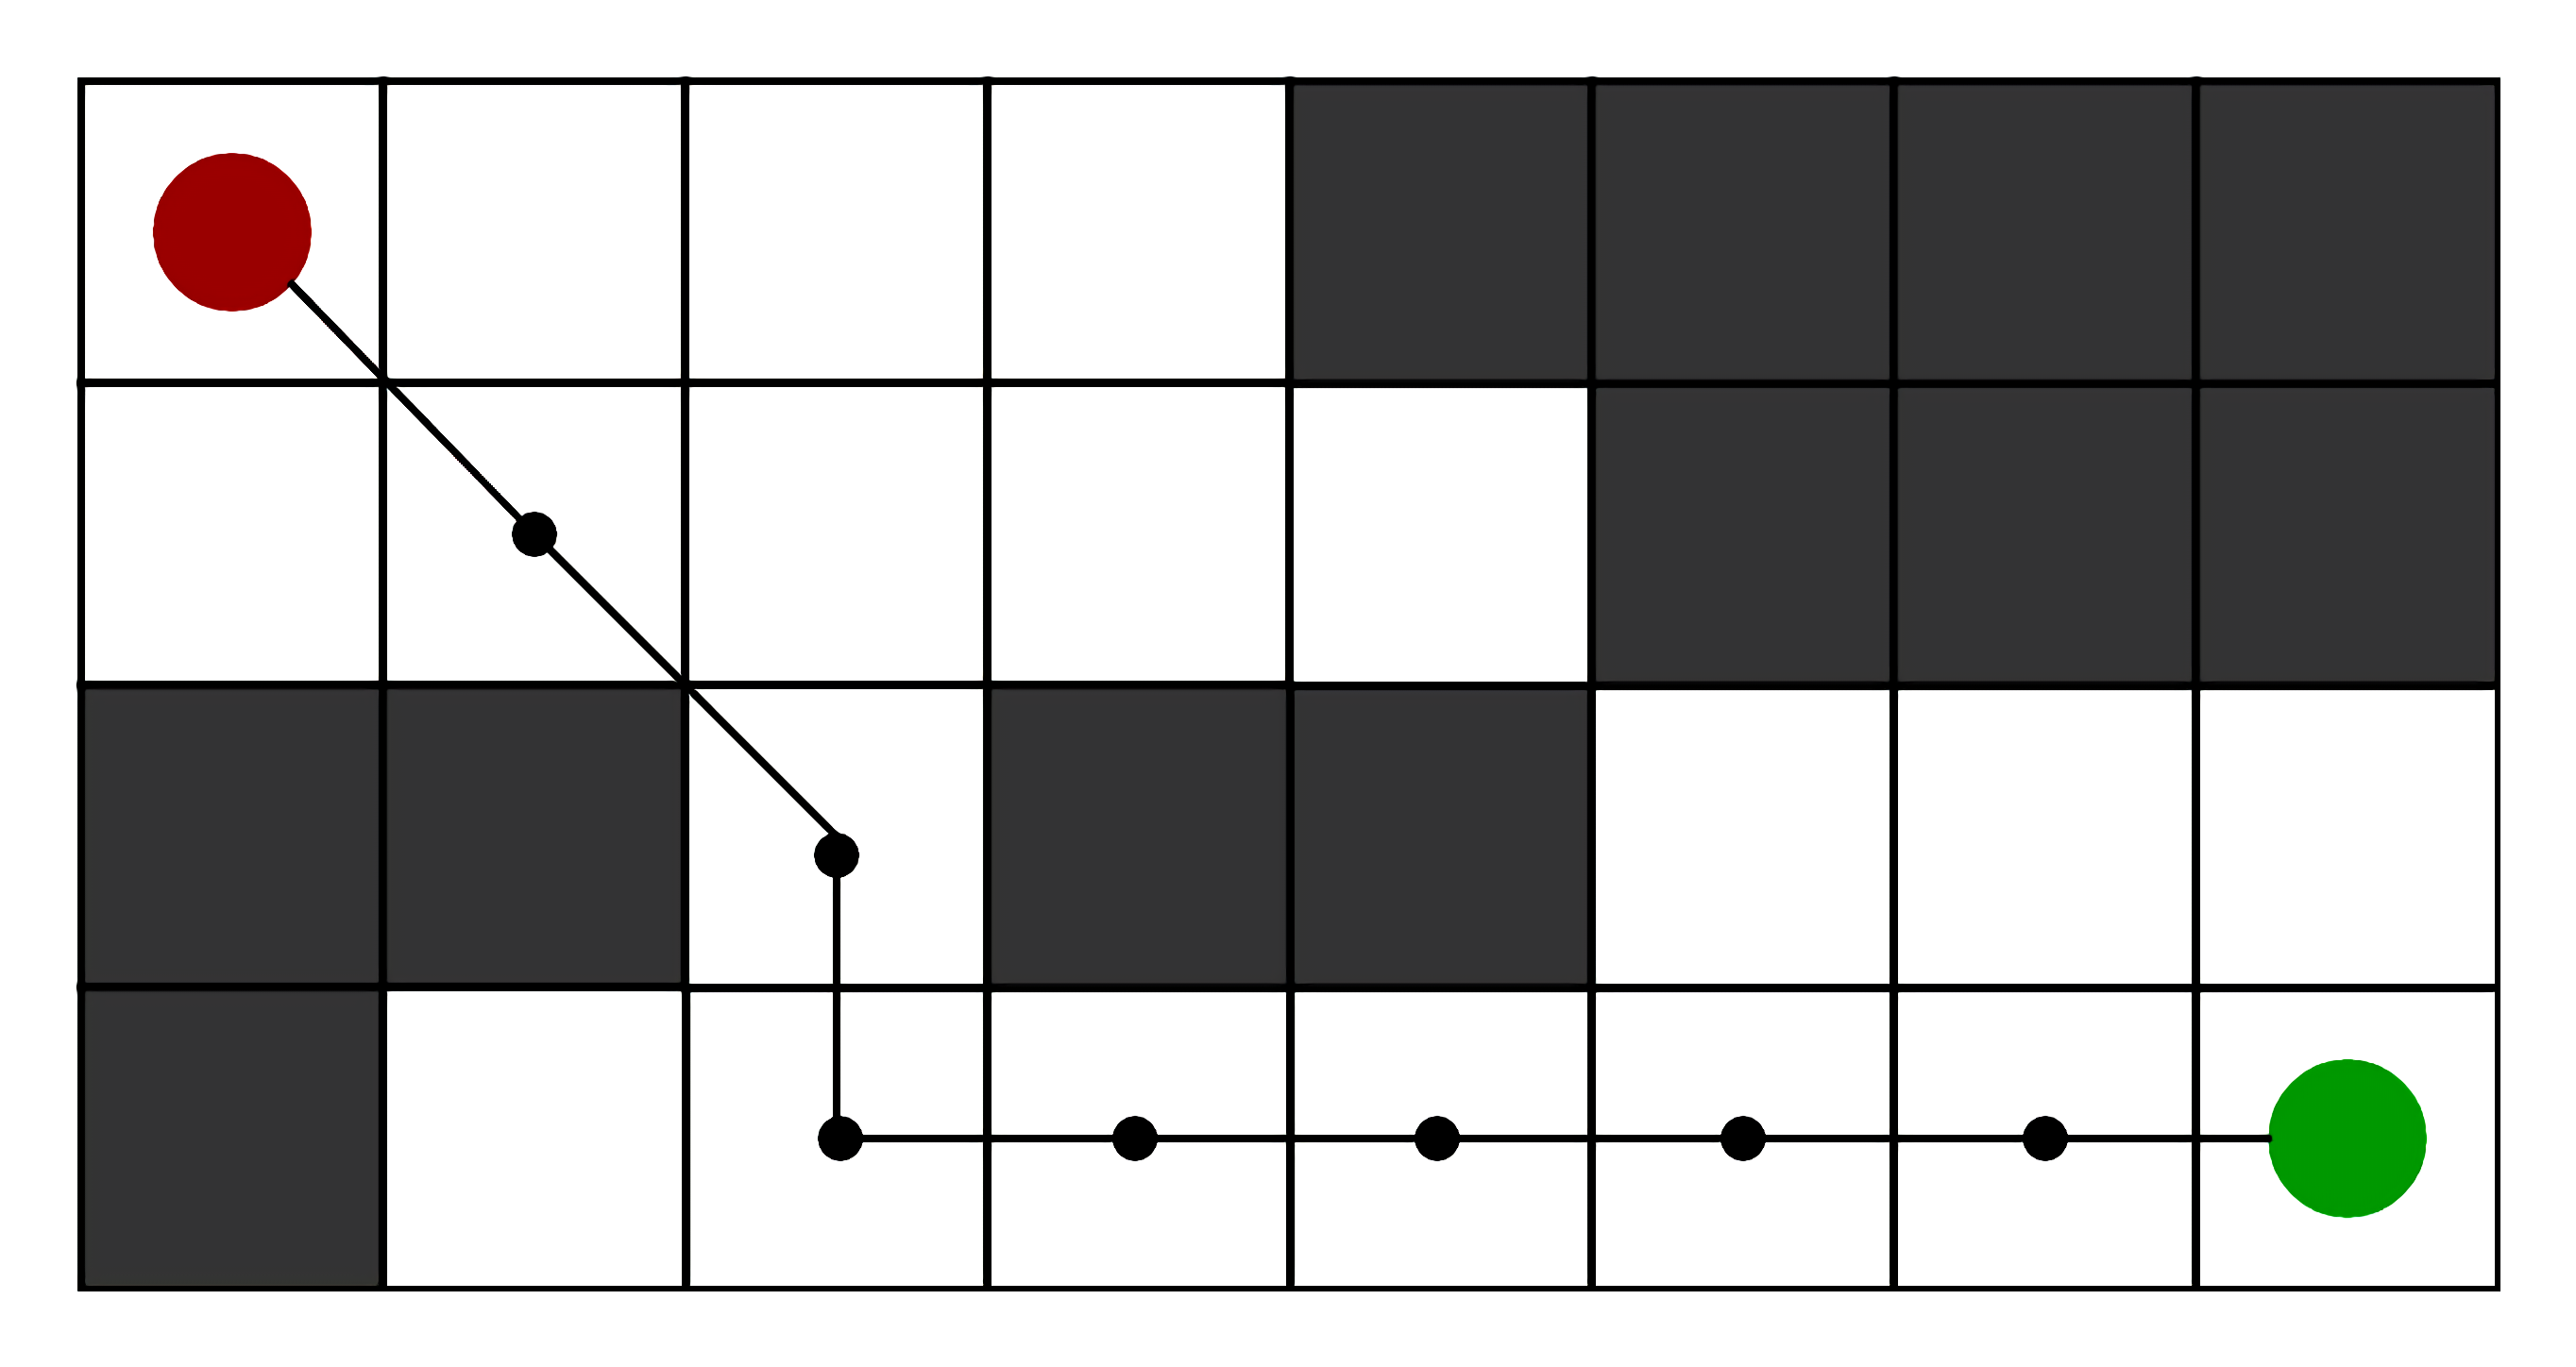
\includegraphics[width=0.8\textwidth]{a-star.png}
    \caption{Pathfinding}
\end{figure}
\end{frame}


\end{document}
